\chapter{Risk Analysis}
The planning of any major project involves certain risks. The larger the project, the more diverse and potentially dangerous the risks are for the success of the project. For this reason, project managers are well advised to do a risk analysis when planning the project in order to identify risks at an early stage and to counter them. The first step is to identify and analyse risks in all areas related to the project.

\section{Risk Identification}
Risks can arise in all areas that have something to do with the project. These include financial risks, risks in time management, human resources and delays in the execution of tasks. External processes such as shortages of suppliers or even the weather can also have an influence on the project and are therefore to be regarded as risks. The risks identified for this project and an estimate of the Probability of Occurence (PoO) are listed in the following table \ref{risk-table}.

\begin{table}[]
	\centering
	\begin{tabular}{|l|l|c|}
		\hline
		\textbf{Risk}                                                                            & \textbf{Description}                                                                                                                                                 & \multicolumn{1}{l|}{\textbf{PoO}} \\ \hline
		\multicolumn{3}{|l|}{\textbf{Human Resources}}                                                                                                                                                                                                                                                     \\ \hline
		Illness                                                                                  & \begin{tabular}[c]{@{}l@{}}The employee is ill and therefore cannot perform \\ his or her tasks as sheduled.\end{tabular}                                           & 0.5                               \\ \hline
		Injury                                                                                   & \begin{tabular}[c]{@{}l@{}}The employee suffers an accident and therefore \\ cannot perform his or her tasks as sheduled.\end{tabular}                              & 0.2                               \\ \hline
		Work Overload                                                                            & \begin{tabular}[c]{@{}l@{}}Too many tasks are assigned to the employee \\ at the same time, so that he or she cannot \\ complete all tasks as planned.\end{tabular} & 0.8                               \\ \hline
		Family problems                                                                          & \begin{tabular}[c]{@{}l@{}}An employee's family member is in need of care \\ and the employee is therefore temporarily absent.\end{tabular}                         & 0.1                               \\ \hline
		\multicolumn{3}{|l|}{\textbf{Financial Problems}}                                                                                                                                                                                                                                                  \\ \hline
		Exceeding the budget                                                                     & \begin{tabular}[c]{@{}l@{}}The realization of the project costs more \\ than planned\end{tabular}                                                                   & 0.3                               \\ \hline
		\multicolumn{3}{|l|}{\textbf{Project Planning and Sheduling}}                                                                                                                                                                                                                                      \\ \hline
		Deadline is too early                                                                    & \begin{tabular}[c]{@{}l@{}}The project does not meet the requirements at \\ the deadline and/or is not completed.\end{tabular}                                      & 0.7                               \\ \hline
		\begin{tabular}[c]{@{}l@{}}Implementation of single \\ tasks takes too long\end{tabular} & \begin{tabular}[c]{@{}l@{}}The implementation of individual tasks is \\ more complex and takes longer than expected\end{tabular}                                    & 0.5                               \\ \hline
		Goal not achived                                                                         & The goal of the project is not achieved.                                                                                                                            & 0.3                               \\ \hline
		\multicolumn{3}{|l|}{\textbf{Delivery}}                                                                                                                                                                                                                                                            \\ \hline
		Insufficient quality                                                                     & \begin{tabular}[c]{@{}l@{}}The quality of the product does not \\ meet the requirements\end{tabular}                                                                & 0.4                               \\ \hline
		\multicolumn{3}{|l|}{\textbf{External Factors}}                                                                                                                                                                                                                                                    \\ \hline
		Shortages of suppliers                                                                   & \begin{tabular}[c]{@{}l@{}}A supplier cannot provide the required \\ quantity of material or equipment at \\ a specified time.\end{tabular}                         & 0.2                               \\ \hline
		Weather                                                                                  & \begin{tabular}[c]{@{}l@{}}The installation of cameras outside \\ the building is delayed by bad weather.\end{tabular}                                              & 0.1                               \\ \hline
	\end{tabular}
	\caption{Identified risks for the project}
	\label{risk-table}
\end{table}

\section{Risk evaluation}
In order to prioritise certain risks so that they can be adequately managed, the risks identified in the previous step must first be estimated for their potential impact on the project.
\begin{figure}[H]
	\centering
	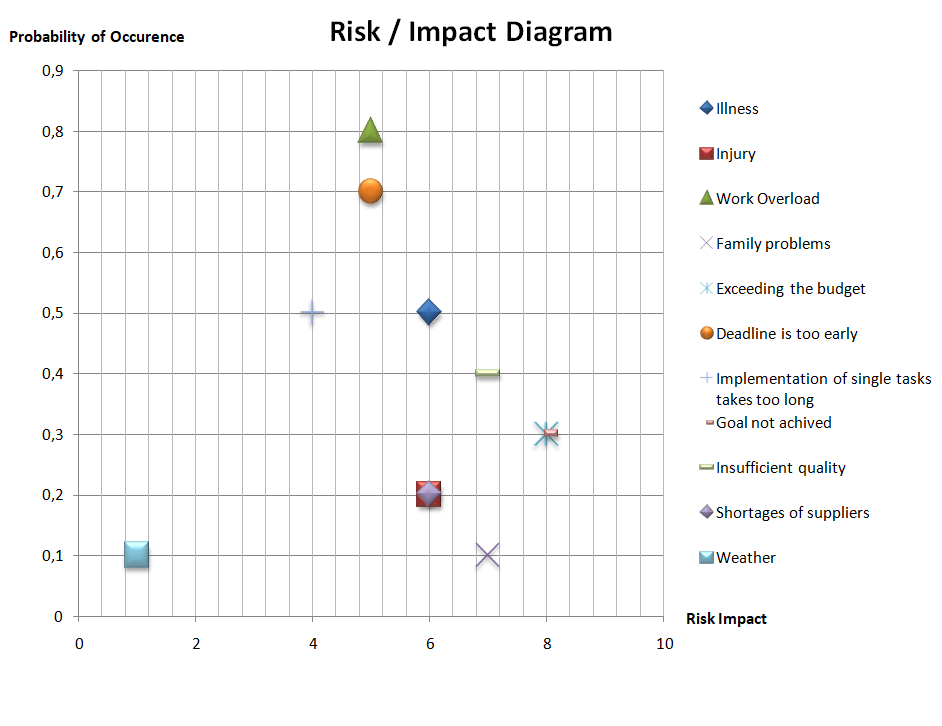
\includegraphics[width =1.1\textwidth]{images/risk-impact2.PNG}
	\caption{Risk/Impact diagram}
	\label{risk-impact}
\end{figure}
The diagram in figure \ref{risk-impact} shows the probability of occurence of the individual risks compared to the possible impact on the project. The impact is evaluated on a scale of 1 to 10. 1 stands for a small but manageable inconvenience, while a 10 represents a threat to the success of the entire project.
\\
As the figure shows, for example, the risk of bad weather poses hardly any threat to the success of the project. A failure to achieve the project's objective however would have far greater impact. Moreover, since the project team consists of only three people, the risks of illness, accidents or other personal problems of the employees were also rated with a large impact. In a project of this size, exceeding the budget would probably have a greater impact on customer satisfaction and thus on the success of the project.

\section{Response to the risk}
If the case described in the risk analysis occurs, it is advisable for the project manager to have a contingency plan in place to reduce the impact on the project. This plan should maintain appropriate measures that do not put too much pressure on the project's employees.
\\
In order to minimize financial or time-related risks, it is necessary to estimate them as precisely as possible in the planning phase at the beginning of the project. If, however, the project cannot be completed within the specified time period or if the budget is exceeded, further negotiations with the customer are necessary in order to develop a solution together.
\\\\
An employee's absence or work overload can only be compensated for by involving colleagues. Each employee should have a deputy who is familiar with the tasks and can take over these tasks if the employee is absent or cannot handle all of his assigned tasks in time. 
\\
For this purpose, there are techniques such as the \textbf{responsibility assignment matrix} (also known as \textbf{RACI} matrix for \textbf{R}esponsible, \textbf{A}ccountable, \textbf{C}onsulted, and \textbf{I}nformed), which can help to distribute responsibilities for certain tasks among several employees. In this matrix, the responsibilities for the individual tasks of the individual employees can be defined using the' R' column. In addition, the' A' column can be used to specify who is accountable for the task to be completed. This allows us to specify a deputy for the task. In addition, it is possible to specify which employees can be consulted in order to fulfil this task and which employees should be informed when the task is completed. Figure \ref{risk-impact} shows a screenshot of the RACI matrix for this project. This matrix was also created using Planhammer's online tool (see chapter \ref{sec:org8452a3e}).
\begin{figure}[H]
	\centering
	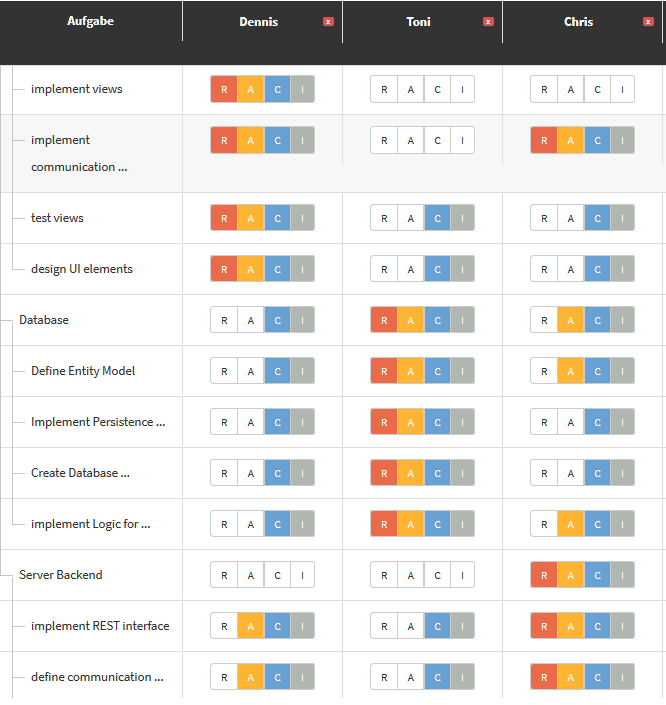
\includegraphics[width =1.0\textwidth]{images/raci.PNG}
	\caption{RACI matrix for the project}
	\label{raci}
\end{figure}